\documentclass[fleqn,xcolor=dvipsnames,8pt]{beamer} % en min\'uscula!
\usefonttheme{serif} % fuentes de LaTeX
\usetheme{Luebeck} % tema escogido en este ejemplo
\usefonttheme{professionalfonts}
%\setbeamercovered{transparent=0}
\usecolortheme[RGB={3,141,182}]{structure}
\setbeamertemplate{navigation symbols}{}
%%%% packages y comandos personales %%%%
\usepackage[utf8]{inputenc}
\usepackage[T1,OT1]{fontenc}
\usepackage[subsection]{algorithm}
\usepackage{algorithmic}
\usepackage{graphicx}
\usepackage[spanish]{babel}
%\usepackage{anyfontsize}
\usepackage{amsfonts,amsmath,amssymb} % S\'imbolos

%\usepackage{epsfig, subfigure}
%\floatname{algorithm}{Procedure}
%\renewcommand{\algorithmicrequire}{\textbf{Input:}}
%\renewcommand{\algorithmicensure}{\textbf{Output:}}
%\selectlanguage{spanish}
\renewcommand{\refname}{Bibliografía}
\hypersetup{
	pdftitle ={Matlab with Arduino},
	pdfauthor ={Edwin Christian Yllanes Cucho},
	pdfsubject ={Propuesta},
	pdfkeywords ={}
}
\begin{document}
\title{Applications with Matlab and Arduino}
\author[Edwin Yllanes]{{\large Edwin Yllanes}\\ Email: \texttt{e.yllanescucho@ieee.org}}
\date{
\includegraphics[width=0.9\textwidth]{images/logo.jpg}}
\begin{frame}
\titlepage
\end{frame}
\begin{frame}
\tableofcontents
\end{frame}
\section{Conceptos Previos}
\subsection{GUIDE}
\begin{frame}{GUIDE: GUI design environment}
\begin{figure}
\centering
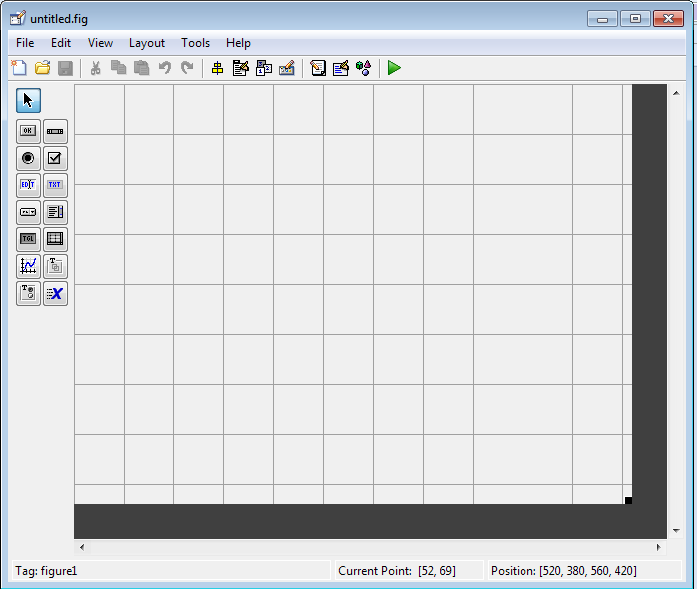
\includegraphics[height=0.6\textheight]{images/guide.png}
\caption{GUIDE}
\end{figure}
\end{frame}
\subsection{Arduino}
\begin{frame}{Arduino}
\end{frame}
\subsection{Materiales}
\begin{frame}{Materiales}
\begin{itemize}
\item Matlab
\item Arduino
\item HCSR04
\item MQ2
\item MQ3
\item PIR
\item DHT22
\end{itemize}
\end{frame}
\section{Proyectos}
\subsection{Radar}
\begin{frame}{Radar}
\begin{figure}
\centering
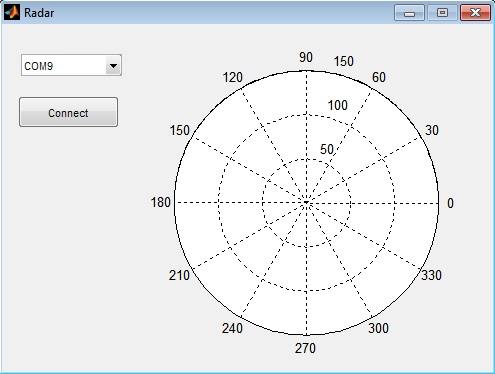
\includegraphics[height=0.6\textheight]{images/radar.png}
\caption{Radar}
\end{figure}
\end{frame}

\begin{frame}{Referencias}
\begin{thebibliography}{1}
\bibitem{Arulampalam}
Arulampalam, M.S.; Maskell, S.; Gordon, N.; Clapp, T.", A tutorial on particle filters for online nonlinear/non-Gaussian Bayesian tracking," Signal Processing, IEEE Transactions on , vol.50, no.2, pp.174,188, Feb 2002
\end{thebibliography}
\end{frame}
\begin{frame}[plain]

  \begin{columns}
    \begin{column}{0.4\textwidth}
      \begin{center}
        %\pgfimage[width=\textwidth]{image/thankyou.jpeg}          
      \end{center}
    \end{column}
    \begin{column}{0.75\textwidth}
      \begin{center}

        \font\endfont = cmss10 at 10.40mm
        \color{Blue}
        \endfont 
        \baselineskip 20.0mm

        Gracias!!!

      \end{center}    

    \end{column}
  \end{columns}

\end{frame}
\end{document}
